\documentclass[a4paper]{article}

\usepackage[portuguese]{babel}
\usepackage[utf8]{inputenc}
\usepackage{indentfirst}
\usepackage{graphicx}
\usepackage{verbatim}
\usepackage{url}
\usepackage{hyperref}

\bibliographystyle{plain}


\begin{document}

\setlength{\textwidth}{16cm}
\setlength{\textheight}{22cm}

\title{\Huge\textbf{Redes Neuronais para a Predição da Origem Geográfica de Música}\linebreak\linebreak\linebreak
\Large\textbf{Relatório Final}\linebreak\linebreak
\linebreak\linebreak

\includegraphics[scale=0.1]{feuplogo.png}\linebreak\linebreak
\linebreak
\Large{Mestrado Integrado em Engenharia Informática e Computação} \linebreak\linebreak
\Large{Inteligência Artifical}\linebreak
}

\author{\textbf{Grupo E4\_1:}\\ Gabriel Souto - 201208167 - ei12087@fe.up.pt \\ José Cardoso - 201202838 - ei12027@fe.up.pt \\\linebreak\linebreak \\
 \\ Faculdade de Engenharia da Universidade do Porto \\ Rua Roberto Frias, s\/n, 4200-465 Porto, Portugal }
\pagebreak


\maketitle
\thispagestyle{empty}

%************************************************************************************************

\newpage

%%%%%%%%%%%%%%%%%%%%%%%%%%
\section{Objectivo}

O objetivo deste trabalho consiste na aplicação de Redes Neuronais Artificiais na predição da origem geográfica de música, recorrendo ao algoritmo de \textit{Back-Propagation}.\linebreak
A partir de um conjunto de exemplos, é possível treinar uma Rede Neuronal, para que esta depois possa ser usada na classificação de novos casos.

%%%%%%%%%%%%%%%%%%%%%%%%%%%%%%%%%%
\section{Especificação}
Para se conseguir atingir o objectivo anteriormente referido, é preciso uma compreensão do \textit{dataset} que iremos usar, fornecido pelo \textit{UCI Machine Learning Repository} \href{http://tinyurl.com/qcxjzap}{aqui}. Este é composto por dois ficheiros que contêm informação de 1059 músicas oriundas de 33 países. O primeiro ficheiro contém 70 atributos, sendo os 68 primeiros atributos obtidos por uma análise das músicas, enquanto que os dois últimos contêm as coordenadas geográficas da capital do país a que pertencem. O segundo ficheiro contém 118 atributos, tendo-se adicionado aos atributos do ficheiro anterior uma análise cromática da música (as coordenadas geográficas continuam a ser os 2 últimos atributos). \linebreak
A nossa abordagem consistiu da seguinte forma: primeiro implementar a rede neuronal, depois o algoritmo e no fim a \textit{gui}. Para representação de conhecimento, representamos cada um dos atributos fornecidos (excluindo os da posição geográfica) como um neurónio da camada de \textit{input}. A camada de \textit{output} é constituída por 33 neurónios, representando cada neurónio 1 país. Os neurónios iriam representar um país de acordo com a primeira vez que ele aparecesse no ficheiro, ou seja, a primeira música no ficheiro irá ter sempre como correcta saída o primeiro neurónio. Na camada de \textit{output}, é suposto um e apenas um neurónio ter o valor a 1 enquanto que os restantes devem ter o seu valor a 0.\linebreak
O algoritmo usado foi o de retro-propagação. Este treina a rede da seguinte forma:

\begin{itemize}
\item Recebe os dados na camada de \textit{input}, propagando-os para as camadas seguintes até os valores chegarem à camada de saída;
\item  Calcula o erro (diferença entre os resultados obtidos e esperados) para cada neurónio na camada de saída, retro-propagando-os até à primeira camada interna;
\item Actualiza os pesos de acordo com o erro de cada neurónio;
\item Repetir até o erro da rede ser baixo o suficiente.
\end{itemize}



%%%%%%%%%%%%%%%%%%%%%%%%%%%%%%
\section{Desenvolvimento}

Este trabalho foi desenvolvido em java, usando-se o IDE \textit {eclipse} e o SO \textit{windows}.

A nossa aplicação foi dividida em 4 \textit{packages} (Figura 1): 
\begin{itemize}
\item  \textit{neural}, que contém a lógica da aplicação (Figura 2);
\item  \textit{test}, que contém uma classe de teste em \textit{JUnit4};
\item \textit{fileReader}, que contém uma classe que lê o ficheiro com os \textit{inputs} de treino;
\item \textit{gui}, que contém a interface gráfica (Figura 3).
\end{itemize}


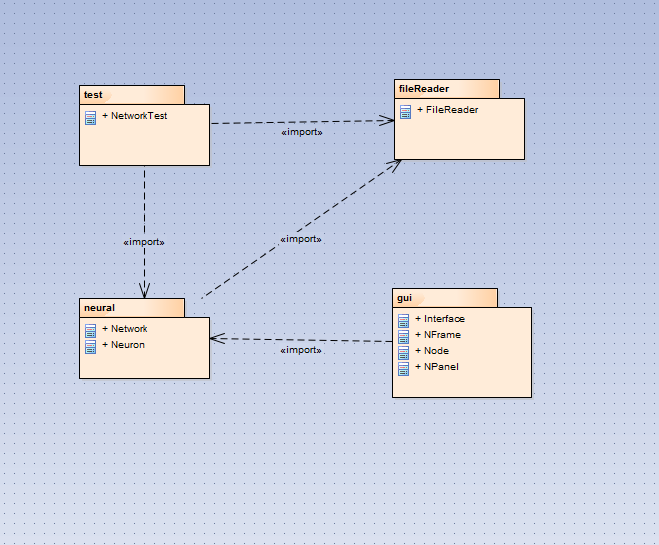
\includegraphics[scale=0.5]{packages.png}
\\Figura 1: Diagrama de pacotes\linebreak\linebreak




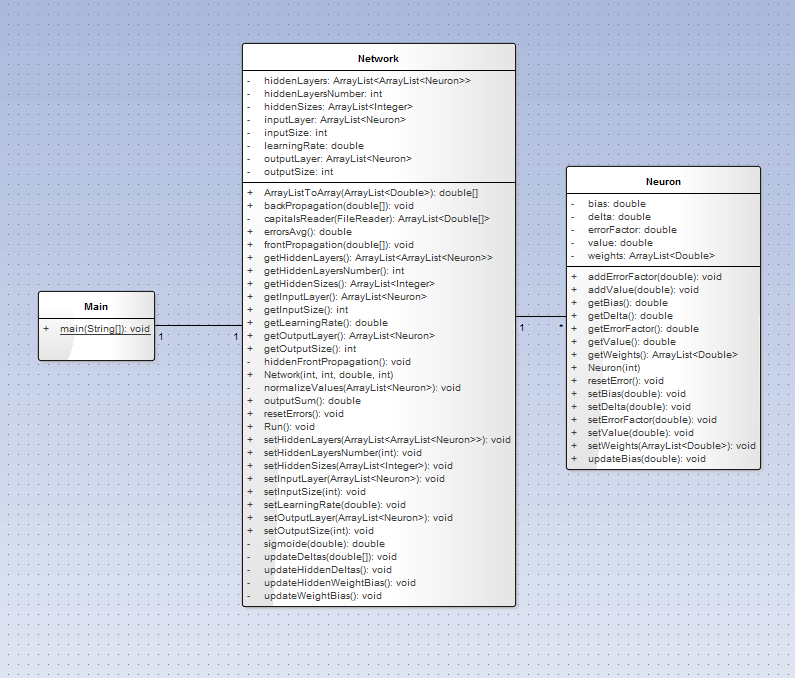
\includegraphics[scale=0.5]{neural.png}
\\Figura 2: Diagrama do pacote neural\linebreak\linebreak


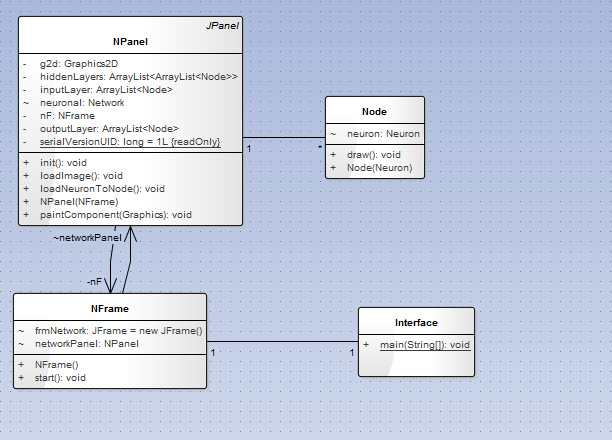
\includegraphics[scale=0.5]{gui.png}
\\Figura 3: Diagrama do pacote gui\linebreak\linebreak

O trabalho desenvolveu-se da seguinte forma: \linebreak
Primeiramente, tratou-se da criação da rede neuronal em si (de acordo com os inputs fornecidos), ou seja, das camadas, dos neurónios e dos pesos.\linebreak
Segundamente, tratou-se da implementação da parte de \textit{frontpropagation} do algoritmo, ou seja, das funções de somatório e de transeferência.\linebreak
Terceiramente, tratou-se de implementar a parte de \textit{backpropagation} do algoritmo, ou seja, do cálculo do erro e do acerto dos pesos.\linebreak
Por fim, tratou-se de implementar da parte gráfica.

\section{Experiências}
Experiências com o ficheiro sem atributos cromáticos:

Experiência 1: Correr o ficheiro com apenas 1 música, um número aleatório de vezes
Resultado: Todos os neurónios na camada de saída com um valor próximo de 0, excepto o um deles cujo resultado é próximo de 1.

Experiência 2: Correr o ficheiro com todas as músicas, um número aleatório de vezes
Resultado: Todos os neurónios na camada de saída ficam com um valor próximo de 0


Experiências com o ficheiro com atributos cromáticos:

Experiência 1: Correr o ficheiro com apenas 1 música, um número aleatório de vezes
Resultado: Todos os neurónios na camada de saída com um valor próximo de 0, excepto um deles cujo resultado é próximo de 1.

Experiência 2: Correr o ficheiro com todas as músicas, um número aleatório de vezes
Resultado: Todos os neurónios na camada de saída ficam com um valor próximo de 0

Experiência 3: Correr o ficheiro com 2 músicas, um número aleatório de vezes
Resultado do 1º Input: Dois neurónios tendem para 1, os restantes tendem para 0 
Resultado do 2º Input: O neurónio correcto com um valor próximo de 1, os restantes neurónios com um valor próximo de 0


%%%%%%%%%%%%%%%%%%%%%%%%%%
\section{Conclusões}
Com estes resultados foi possível concluir que a rede neuronal implementada não é capaz de resolver o problema proposto, com um número de \textit{inputs} grande. 


%%%%%%%%%%%%%%%%%%%%%
\section{Melhoramentos}

Como a nossa rede não consegue aprender e ser treinada para um numero elevado de inputs, como podemos verificar pelas experiências, uma melhoria para o futuro seria descobrir o porquê disto. Ou seja, descobrir o passo da implementação do algoritmo que não se encontra completamente correcto, corrigí-lo e verificar os resultados obtidos através de utilizações de \textit{framework} prórias como o \textit{Weka}.
Outra melhoria seria melhorar a visualização gráfica da rede, tornando mais interactiva visto que esta é uma representação estática do resultado final do algoritmo. Um exemplo seria fazer com que fosse possível ver cada iteração do mesmo ou fazer com que os neurónios pudessem ser movidos.


%%%%%%%%%%%%%%%%%%%%%%%%%%
\section{Recursos}

[1] Fang Zhou, Claire Q and Ross. D. King. Predicting the Geographical Origin of Music, ICDM.
\url{http://archive.ics.uci.edu/ml/datasets/Geographical+Original+of+Music}, 2014

\clearpage


%%%%%%%%%%%%%%%%%%
\section{Apêndice}
O nosso projecto é constituído por 2 modos de utilização distintos, uma interface pela consola e outra gráfica.

A interface pela consola é acedida através do IDE eclipse, executando o codigo apartir da classe NetworkTest.java. Esta é constituida por uma série de testes unitarios, sendo o ultimo a execução completa da rede neuronal.

A interface gráfica é acedida através do IDE eclipse, executando o código apartir da classe Interface.java do package GUI. Esta consiste num menu inicial, no qual o utilizador pode escolher o número de valores de input, output e learning rate. O utilizador também deve selecionar o dataset pretendido através do botão “Load Dataset” que abrirá um file explorer para aceder ao ficheiro pretendido. Depois de isto tudo estar configurado, o utilizador deve clicar no botão “start” e aí ser-lhe-ão apresentados os neurónios, cada um com o seu valor, organizados em camadas codificadas por cor ( Preto para camada de input, Azul para as camadas e intermedias, e Verde ou Vermelho para a camada de output conforme seja o valor se aproxime de 0 (vermelho) ou 1 (verde)).

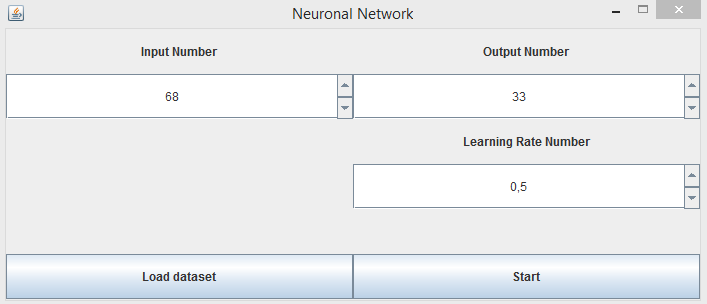
\includegraphics[scale=0.5]{client.png}
\\Figura 4: Interface gráfica\linebreak\linebreak

\end{document}
